\chapter{Unità logaritmiche} 

\begin{figure}[h]
    \centering
    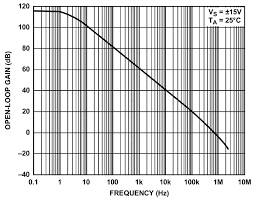
\includegraphics[scale = 1]{Operazionale in db.jpg}
\end{figure}  

\newpage 

\section{Breve appendice sulle unità logaritmiche} 

Per esprimere guadagni e attenuazioni, nonchè cifre di rumore e rapporti segnale rumore, 
si usano frequentemente le unità logaritmiche. \newline 

Se consideriamo due segnali $A_1$ e $A_2$, in db diventeranno:

{
    \Large 
    \begin{equation}
        \left. (\frac{A_1}{A_2}) \right|_{db} 
        = 20 \cdot \log_{10} (\frac{A_1}{A_2})
    \end{equation}
}

Nel caso di due potenze $P_1$ e $P_2$: 

{
    \Large 
    \begin{equation}
        \left. (\frac{P_1}{P_2}) \right|_{db} 
        = 10 \cdot \log_{10} (\frac{P_1}{P_2})
    \end{equation}
}


L'uso dei db è molto utile perchè semplifca le operazioni di questo tipo:

{
    \Large 
    \begin{equation}
        \log(X^{\alpha}) = \alpha \cdot \log X 
    \end{equation}
}

{
    \Large 
    \begin{equation}
        \log(X_1 \cdot X_2) = \log X_1 +  \log X_2 
    \end{equation}
}

{
    \Large 
    \begin{equation}
        \log(\frac{X_1}{X_2}) = \log X_1 -  \log X_2 
    \end{equation}
}

Le proprietà appena elencate valgono per qualsiasi base usata nei logaritmi. \newline 

Se una grandezza è dimensionale ed è espressa in unità assolute (ad esempio una potenza P espressa in W), allora, possiamo convertirla in db: 

{
    \Large 
    \begin{equation}
        (P)_{dbW} = 10 \cdot \log_{10}[(P)_W]
    \end{equation}
} 

Se invece la voglia in milli Watt (mW) in db, avremo che: 

{
    \Large 
    \begin{equation}
        (P)_{dBm} = 10 \cdot \log_{10}[(P)_{mW}]
    \end{equation}
}

Data una potenza P, possiamo scrivere questa relazione: 

{
    \Large 
    \begin{equation}
        (P)_{dBm} = (P)_{dBW} + 30
    \end{equation}
} 

\newpage
.
\newpage
. 
\newpage